\subsubsection{conform} \label{sec:conform}

The operation \operator{conform} identifies a reachset-conformant model (see \cref{sec:isconform} for a detailed explanation of reachset conformance). Depending on our prior knowledge about the model, we can solely identify the uncertainty sets, which make the model reachset-conformant, (termed white-box identification) or we can also identify unknown model parameters (gray-box identification) or the whole model dynamics (black-box identification)~\cite{Luetzow2024a,Luetzow2024b}.
Reachset conformance has been established in numerous applications, such as safe human-robot co-existence~\cite{Liu2017a}, safe robot manipulators \cite{Liu2018a}, force control \cite{Liu2021c}, and analog circuits \cite{Kochdumper2020b}.

\begin{table}[h]
	\caption{Conformance identification algorithms.}
	\centering
	\label{tab:confAlg}
	\begin{tabular}{l p{9cm} l}
		\toprule
		\textbf{Algorithm} & \textbf{Description} & \textbf{Reference} \\
		\midrule
		\texttt{white} & identification of the scaling factors and (for linear systems) center vectors of the uncertainty sets, which make a given model reachset-conformant, with linear programming & \cite{Luetzow2024a} \\
		\texttt{graySim} & simultaneous identification of the uncertainty sets and unknown model parameters with nonlinear programming. & \cite{Luetzow2024b} \\
		\texttt{graySeq} & sequential identification of unknown model parameters and the uncertainty sets with nonlinear programming. & \cite{Luetzow2024b} \\
		\texttt{grayLS} & sequential identification of unknown model parameters and the uncertainty sets with nonlinear programming using least squares cost function. &  \cite{Luetzow2024b} \\
		\texttt{blackCGP} & identification of a reachset-conformant model using conformant genetic programming. &  \cite{Luetzow2024b} \\
		\texttt{blackGP} & identification of a reachset-conformant model using standard genetic programming & \cite{Luetzow2024b} \\
		\texttt{RRT} & increase additive uncertainty sets until all trajectories, generated with rapidly exploring random trees (RRTs), are contained in the reachable set of the model. & \cite{Althoff2012b} \\
		\bottomrule
	\end{tabular}
\end{table}

The syntax for the operation \texttt{conform} is:
\begin{equation*}
\begin{split}
    & [\texttt{params}, \texttt{results}] = \texttt{conform}(\texttt{sys},\texttt{params},\texttt{options},\texttt{type})
\end{split}
\end{equation*}
with input arguments

\begin{center}
\renewcommand{\arraystretch}{1.3}
\begin{tabular}[t]{l p{13cm} }
	$\bullet$~\texttt{sys} & dynamic system defined by one of the classes \texttt{linearSysDT} (see \cref{sec:linearSysDT}), \texttt{linearARX} (see \cref{sec:linearARX}), \texttt{nonlinearSysDT} (see \cref{sec:nonlinearSystemsDT}), or \texttt{nonlinearARX} (see \cref{sec:nonlinearSystems_ARX}). \\
	$\bullet$~\texttt{params} & struct containing the parameter that define the conformance problem. \\
	& \begin{tabular}[t]{l p{10cm}}
	 	--~\texttt{.tStart} & initial time $t_0$ (default value 0). \\
	 	--~\texttt{.tFinal} & final time $t_f$. \\
	 	--~\texttt{.R0} & initial uncertainty set ${\mathcal{X}}_0$ relative to the initial state, specified as an object of class \texttt{zonotope} (see \cref{sec:zonotope}).\\
	 	--~\texttt{.U} & initial uncertainty set $\mathcal{U}$ relative to the input, specified as an object of class \texttt{zonotope} (see \cref{sec:zonotope}). \\
	 	--~\texttt{.testSuite} & cell array of testCase objects, which contain input trajectories and the corresponding output trajectories of the implementation system $S_I$.
	 \end{tabular}
\end{tabular}
\begin{tabular}[t]{l p{13cm} }
	$\bullet$~\texttt{options} & struct containing algorithm settings for conformance synthesis. For the white-, gray-, and black-box identification algorithms, we can specify:  \\
	& \begin{tabular}[t]{l p{10cm}}
		--~\texttt{.cs.cost} & cost function for reachset conformance synthesis, currently the interval norm (\texttt{interval}) and the Frobenius norm (\texttt{Frob}) are supported (see \cite{Althoff2023a}). \\
		--~\texttt{.cs.w} & weighting vector for the norm at different times for reachset conformance synthesis, the default value is a vector of ones. \\
		--~\texttt{.cs.P} & weighting matrix for the Frobenius norm, the default value is the identity matrix. \\
		--~\texttt{.cs.constraints} & type of containment constraints, currently halfspace constraints (\texttt{half}) and generator constraints (\texttt{gen}) are supported (see \cite{Luetzow2024a}). \\
		--~\texttt{.cs.robustnessMargin} & robustness value for enforcing the containment constraints, the default value is $1e-9$. \\
		--~\texttt{.cs.derivRecomputation} & boolean, which can enforce the Jacobian and Hessian recomputation (required for linearization) at each nonlinear programming iteration.\\
		--~\texttt{.cs.a\_min} & lower limit for the identified scaling factors, default is $0$. \\
		--~\texttt{.cs.a\_max} & upper limit for the identified scaling factors, default is $\infty$. \\
		--~\texttt{.cs.cp\_lim} & upper limit for the absolute value of the identified center vectors and parameters, default is $\infty$. \\
		--~\texttt{.cs.verbose} & boolean, which can suppress displaying output.
	\end{tabular}
\end{tabular}
\begin{tabular}[t]{l p{13cm} }
 & For the gray-box algorithms, \texttt{options} can also contain:  \\
 & \begin{tabular}[t]{l p{10cm}}
	--~\texttt{.cs.p0} & initial estimate for the parameters. \\
	--~\texttt{.cs.set\_p} & function handle, which return the system object and the uncertainty sets for a given parameter vector (default: parameter vector contains the center vectors of the uncertainty sets). \\
	--~\texttt{.cs.p\_min} & lower limits for the parameter vector, default is \texttt{options.cs.p0}$-$\texttt{options.cs.cp\_lim}. \\
	--~\texttt{.cs.p\_max} & upper limits for the parameter vector, default is \texttt{options.cs.p0}$+$\texttt{options.cs.cp\_lim}. \\
	--~\texttt{.cs.cp\_lim} & upper limit for the absolute value of the identified center vectors and parameters, default is $\infty$. \\
	--~\texttt{.cs.timeout} & time in $s$ after which the nonlinear programming solver is forced to stop.
\end{tabular}\\
	& For the black-box algorithms, we can also specify a large number of settings for the genetic programming approach. A list can be found in the file \texttt{config\_contDynamics\_conform\_black}.  \\
	$\bullet$~\texttt{type} & algorithm type (see \cref{tab:confAlg}); can be omitted for \texttt{white}.
\end{tabular}
\end{center}

and output arguments

\begin{center}
\renewcommand{\arraystretch}{1.3}
\begin{tabular}[t]{l p{13cm} }
    $\bullet$~\texttt{params} & struct containing the updated uncertainty sets \\
	$\bullet$~\texttt{results} & struct with the optimization results, which depend on the algorithm type and can be: \\
	& \begin{tabular}[t]{l p{10cm}}
		--~\texttt{.R} & object of class \texttt{reachSet} (see \cref{sec:reachSet}) that stores the observed set $\mathcal{R}(t_i)$ for all time points if the algorithm is \texttt{RRT}.\\
		--~\texttt{.simRes} & object of class \texttt{simResult} (see \cref{sec:simResult}) that stores simulated trajectories if the algorithm is \texttt{RRT}.\\
		--~\texttt{.fval} & final optimization cost. \\
		--~\texttt{.p} & optimized parameters. \\
		--~\texttt{.sys} & optimized dynamic system. \\
		--~\texttt{.unifiedOutputs} & Methods for linear systems unify outputs using the superposition principle, which are collected in this matrix.
	\end{tabular}
\end{tabular}
\end{center}


Let us demonstrate the operation \texttt{conform} by an example (the plot shows the reachable output set of the conformant model and the measured outputs): 

\begin{center}
\begin{minipage}[t]{\textwidth}
	\footnotesize
	% This file was created by matlab2tikz.
%
\definecolor{mycolor1}{rgb}{0.27060,0.58820,1.00000}%
%
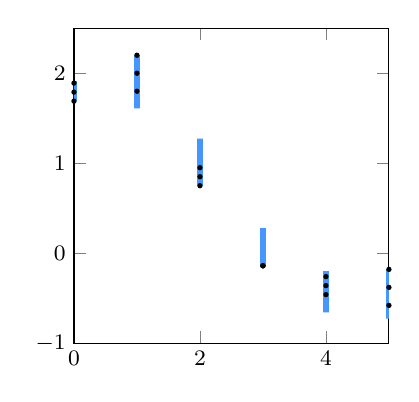
\begin{tikzpicture}
\footnotesize

\begin{axis}[%
width=4cm,
height=4cm,
at={(0in,0in)},
scale only axis,
xmin=0,
xmax=5,
ymin=-1,
ymax=2.5,
axis background/.style={fill=white}
]

\addplot[area legend, line width=2.0pt, draw=mycolor1, fill=mycolor1, forget plot]
table[row sep=crcr] {%
x	y\\
0	1.69\\
0	1.9135\\
}--cycle;

\addplot[area legend, line width=2.0pt, draw=mycolor1, fill=mycolor1, forget plot]
table[row sep=crcr] {%
x	y\\
1	1.6085\\
1	2.2\\
}--cycle;

\addplot[area legend, line width=2.0pt, draw=mycolor1, fill=mycolor1, forget plot]
table[row sep=crcr] {%
x	y\\
2	0.75\\
2	1.2743\\
}--cycle;

\addplot[area legend, line width=2.0pt, draw=mycolor1, fill=mycolor1, forget plot]
table[row sep=crcr] {%
x	y\\
3	-0.14\\
3	0.2776\\
}--cycle;

\addplot[area legend, line width=2.0pt, draw=mycolor1, fill=mycolor1, forget plot]
table[row sep=crcr] {%
x	y\\
4	-0.6566\\
4	-0.2004\\
}--cycle;

\addplot[area legend, line width=2.0pt, draw=mycolor1, fill=mycolor1, forget plot]
table[row sep=crcr] {%
x	y\\
5	-0.7283\\
5	-0.18\\
}--cycle;
\addplot [color=black, only marks, mark=*, mark size=0.7500pt, mark options={solid, black}, forget plot]
  table[row sep=crcr]{%
0	1.79\\
};
\addplot [color=black, only marks, mark=*, mark size=0.7500pt, mark options={solid, black}, forget plot]
  table[row sep=crcr]{%
0	1.89\\
};
\addplot [color=black, only marks, mark=*, mark size=0.7500pt, mark options={solid, black}, forget plot]
  table[row sep=crcr]{%
0	1.69\\
};
\addplot [color=black, only marks, mark=*, mark size=0.7500pt, mark options={solid, black}, forget plot]
  table[row sep=crcr]{%
1	2\\
};
\addplot [color=black, only marks, mark=*, mark size=0.7500pt, mark options={solid, black}, forget plot]
  table[row sep=crcr]{%
1	2.2\\
};
\addplot [color=black, only marks, mark=*, mark size=0.7500pt, mark options={solid, black}, forget plot]
  table[row sep=crcr]{%
1	1.8\\
};
\addplot [color=black, only marks, mark=*, mark size=0.7500pt, mark options={solid, black}, forget plot]
  table[row sep=crcr]{%
2	0.85\\
};
\addplot [color=black, only marks, mark=*, mark size=0.7500pt, mark options={solid, black}, forget plot]
  table[row sep=crcr]{%
2	0.95\\
};
\addplot [color=black, only marks, mark=*, mark size=0.7500pt, mark options={solid, black}, forget plot]
  table[row sep=crcr]{%
2	0.75\\
};
\addplot [color=black, only marks, mark=*, mark size=0.7500pt, mark options={solid, black}, forget plot]
  table[row sep=crcr]{%
3	-0.14\\
};
\addplot [color=black, only marks, mark=*, mark size=0.7500pt, mark options={solid, black}, forget plot]
  table[row sep=crcr]{%
3	-0.14\\
};
\addplot [color=black, only marks, mark=*, mark size=0.7500pt, mark options={solid, black}, forget plot]
  table[row sep=crcr]{%
3	-0.14\\
};
\addplot [color=black, only marks, mark=*, mark size=0.7500pt, mark options={solid, black}, forget plot]
  table[row sep=crcr]{%
4	-0.36\\
};
\addplot [color=black, only marks, mark=*, mark size=0.7500pt, mark options={solid, black}, forget plot]
  table[row sep=crcr]{%
4	-0.46\\
};
\addplot [color=black, only marks, mark=*, mark size=0.7500pt, mark options={solid, black}, forget plot]
  table[row sep=crcr]{%
4	-0.26\\
};
\addplot [color=black, only marks, mark=*, mark size=0.7500pt, mark options={solid, black}, forget plot]
  table[row sep=crcr]{%
5	-0.38\\
};
\addplot [color=black, only marks, mark=*, mark size=0.7500pt, mark options={solid, black}, forget plot]
  table[row sep=crcr]{%
5	-0.58\\
};
\addplot [color=black, only marks, mark=*, mark size=0.7500pt, mark options={solid, black}, forget plot]
  table[row sep=crcr]{%
5	-0.18\\
};
\end{axis}
\end{tikzpicture}%
\end{minipage}
\begin{minipage}[t]{\textwidth}
	\vspace{0pt}
	\centering
	\includetikz{./figures/tikz/contDynamics/example_conform}
\end{minipage}
\end{center}
